\chapter{Shape-from-Silhouette Modeling of Small Bodies}
\label{shape_modeling}
\section{Introduction}
We present an approach to image processing and shape modeling for low resoltuion shape models. This involves real and simulated imagery, edge detection algorithms, and dramatic lighting conditions, 
In this work, the models presented are generated from both simulated and actual mission data sources and compared to the most resolute shape models available for the bodies in question. The method is tested on both a convex and irregular body in order to show how our overlaid silhouette trimming procedure responds to self-shadowing, the presence of concavity, as well as phase angles  projections introduced by the orientation of the sun and camera. This work will be developed as necessary to enable onboard shape model generation, but this paper serves to present and defend the method which uses a process of refinement based on extending the shape along the silhouette cutout in space, and narrowing down the three-dimensional hull through multiple view angles. As the small body community looks to grant more SIMPLEx level missions to asteroids, such as the Janus mission which will rendezvous with a binary system, it is necessary to develop the autonomous onboard navigation capabilities that make those missions possible. 

\section{2D to 3D Mapping of Images to Shapes}
\subsection{Assumptions} 
In it's current formulation, this shape modeling method processes a batch of optical and infrared images taken at a reasonable distance away from a target body. The body does not need to be centered in the frame of the image, nor does it need to be fully lit. The assumptions made in the work to follow include full knowledge of the body frame, beginning with the orientation of the spin pole and further defined by convention. The orientation and location of the camera is known along with its frame, as well as the sun location in the body frame. In actual missions, there is a reasonable track of the spacecraft orientation and location in the inertial (sun-centered) frame, and a state estimate is formed for the body during approach and during ground-based observation campaigns. In this work, perfect certainty of the body location, spacecraft location, and the camera-pointing vector can be assumed.    

\subsection{Simulated Image Procedure}
Simulated images were necessary to test the robustness of our modeling method. The process of generating these images was performed via Blender software {blender} with the goal of recreating conditions of the OSIRIS-REx approach phase to the asteroid Bennu. The shape model was of 6m resolution, sourced from the approach data results given by the OSIRIS-REx mission{Lauretta2019}. Lighting conditions, such as the sun location, were manipulated to match the testing criteria but the inherent qualities were kept constant: a light strength of 5 MW, $0\%$ specularity, and a radius of 1m were suitable to illuminate the target for the purpose of recreating mission-similar conditions. Both a regular and irregular body were tested. The camera dimensions were kept in accordance with the PolyCam on the OSIRIS-REx mission{Rizk2017}.
%insert table outlining PolyCam camera parameters that you had to put into Blender (just fov? also image size/resolution?)



\subsection{Mission Data}
\begin{wrapfigure}[18]{R}{0.5\textwidth}
    \centering
    \captionsetup{justification=centering}
     \begin{subfigure}{0.23\textwidth}
         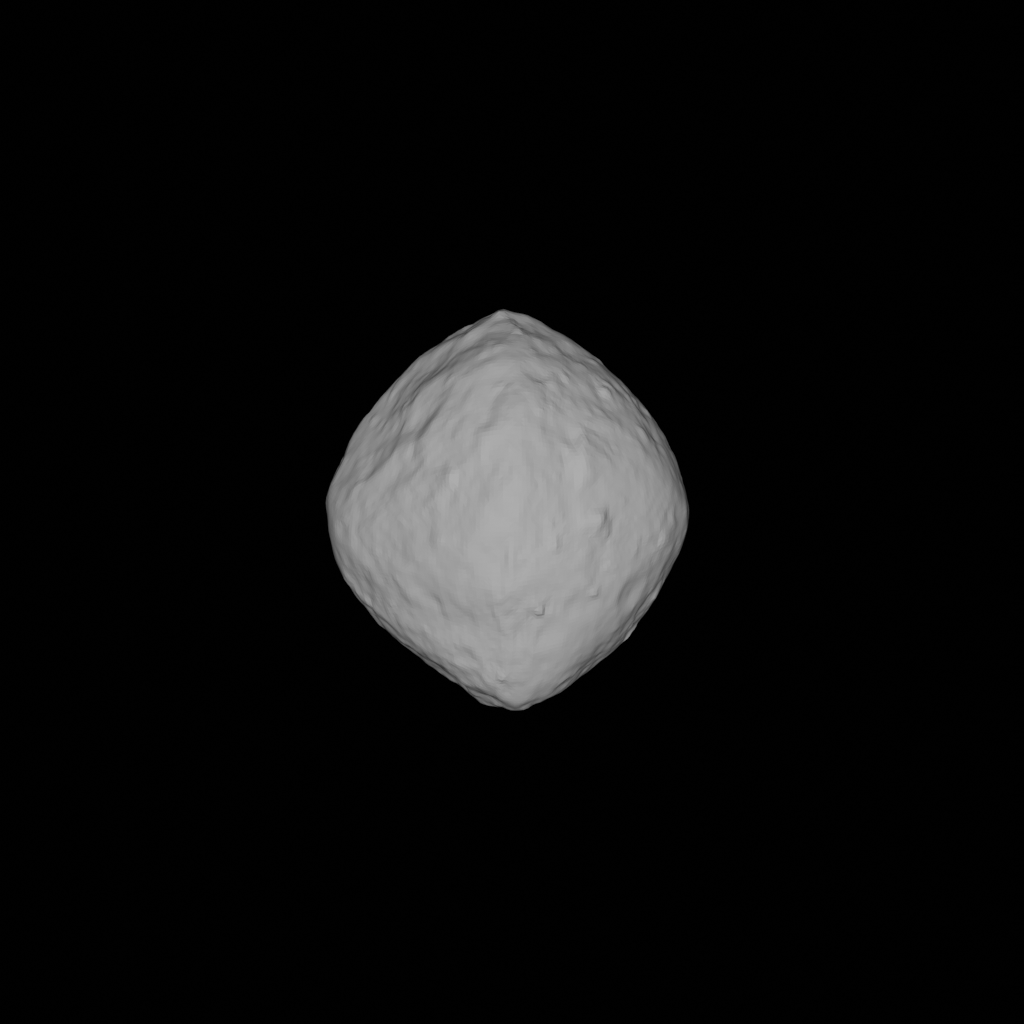
\includegraphics[width =\textwidth, height = \textwidth]{fig/render72.png}
         \caption{Simulated Bennu in Blender}
         \label{fig:y equals x}
     \end{subfigure}
    \hfill
     \begin{subfigure}{0.23\textwidth}
         \centering
         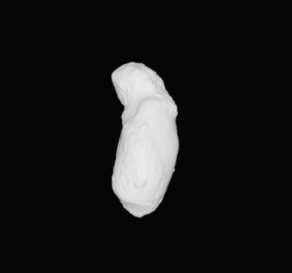
\includegraphics[width = \textwidth, height = \textwidth]{fig/Screen Shot 2021-02-18 at 11.43.43 AM.png}
         \caption{Simulated Itokawa in Blender}
         \label{fig:three sin x}
     \end{subfigure}
     
     \begin{subfigure}{0.23\textwidth}
         \centering
         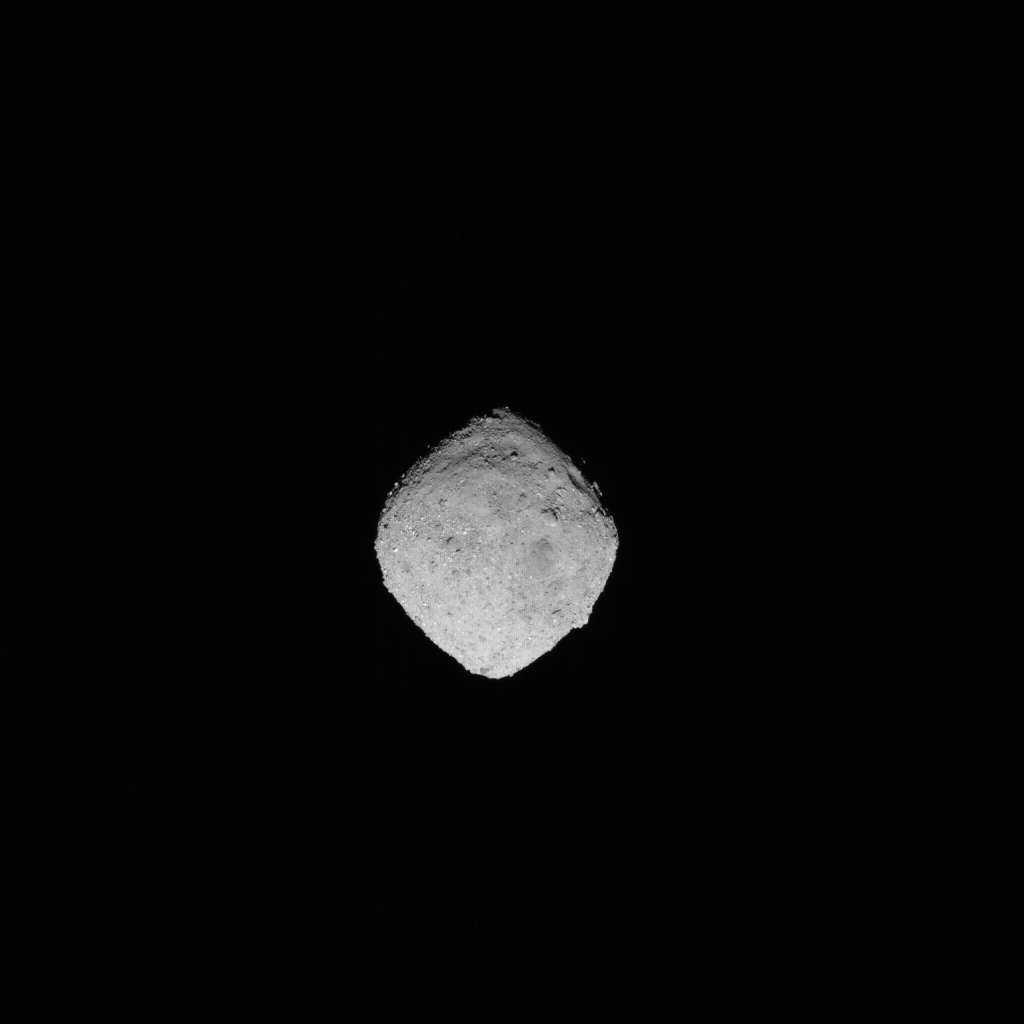
\includegraphics[width=\textwidth, height = \textwidth]{fig/image_69.png}
         \caption{OSIRIS-REx Mission Image}
         \label{fig:y equals x 2}
     \end{subfigure}
    \hfill
     \begin{subfigure}{0.23\textwidth}
         \centering
         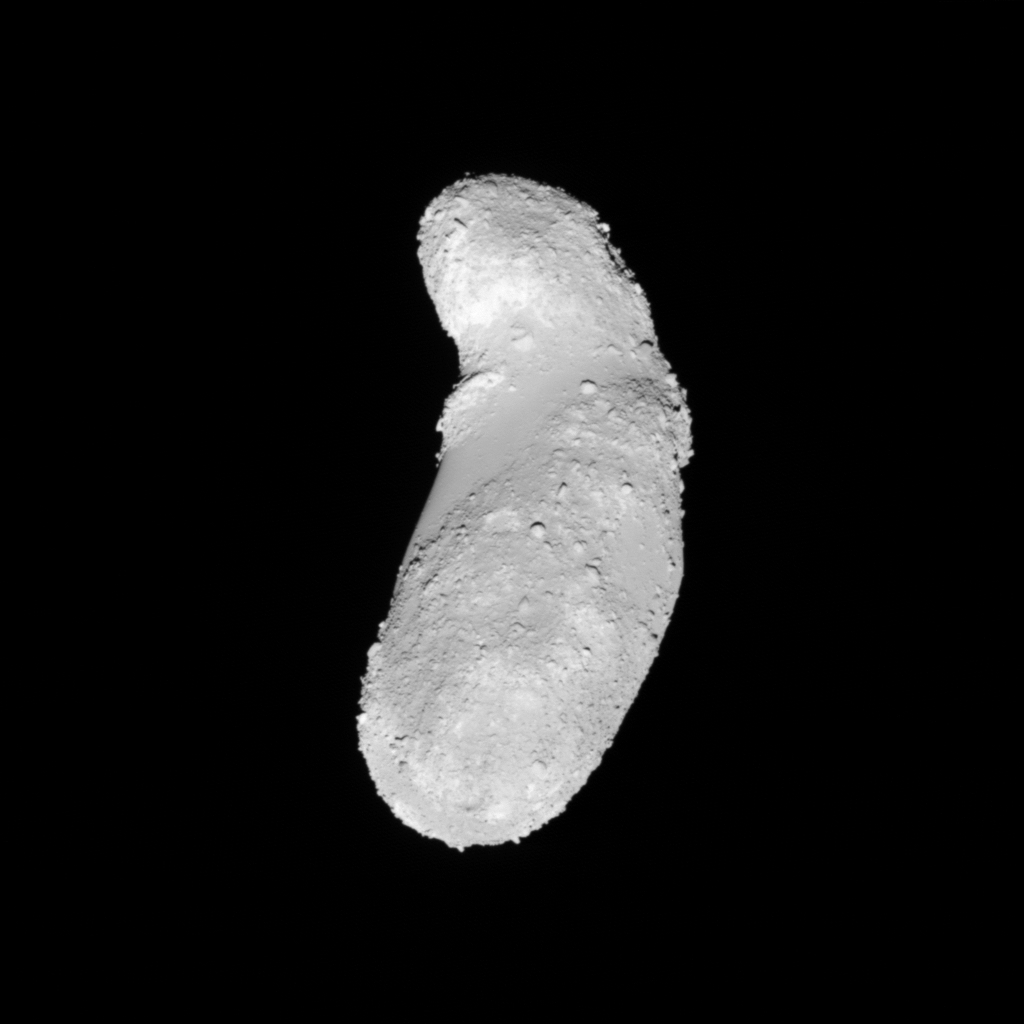
\includegraphics[width=\textwidth, height = \textwidth]{fig/st_2423026558_v.png}
         \caption{Hayabusa Mission Image}
         \label{fig:three sin x 2}
     \end{subfigure}
        \caption{Example Images}
        \label{fig:four_images}
\end{wrapfigure}
The data obtained to further test the modeling software was sourced from the OSIRIS-REx and Hayabusa mission SPICE archives. Necessary data regarding the camera dimensions, frame-to-frame transformations, the state of the camera, body, and sun were accessed as well as the images themselves which came from the PDS archives but their timestamps allowed for coordination of state and image. Shown below is an example of similarity between the simulated image sets and actual mission data, which proves that moving forward with both can provide comparable results when focusing on the silhouette information.



\subsection{Identification of the Silhouette}

The procedure of shape generation using optical data begins with processing the images and finding the desired information - the silhouette of the body. The data shows results where the camera is within 100km, 151km, and 8km of the target body for the simulated test cases, the OSIRIS-REx data, and the Hayabusa images respectively. Examples of the input are shown in Fig. %\ref{fig:four_images}. 
The simulated images and the mission data differ most in their surface detail, where rocks and boulders can be seen readily on mission images but are majorly missing from the surface representations of the shape models processed by Blender. For the purposes of silhouette-based shape modeling, this detail is acceptable and there are many steps implemented to ensure that all data sets are treated equally. This algorithm begins with a pre-processing thresholding procedure. An image is translated from RGB values into grayscale between [0,255] in intensity. These values are then flattened with the lowest intensity pixels ($< 2$) removed and all other intensities amplified by a factor of 1000. This produces a flat background of space with a bright masked featureless image of the body. 
%here insert new thresholded image
\begin{figure}[h!]
\begin{subfigure}{0.4\textwidth}
    \centering
    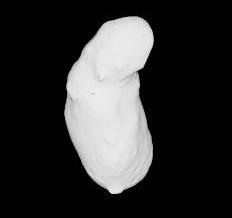
\includegraphics[width = \textwidth, height = 2in]{fig/unproc_ito.jpg}
    \caption{Unprocessed Itokawa Image}
\end{subfigure}
\hfill
\begin{subfigure}{0.4\textwidth}
    \centering
    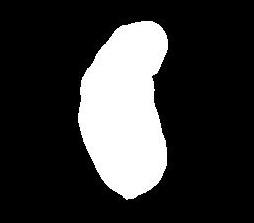
\includegraphics[width = \textwidth, height = 2in]{fig/flat_thresh_ito.jpeg}
    \caption{Processed Itokawa Image}
\end{subfigure}
\end{figure}
\\With a preprocessed, thresholded image, the next step is to apply an edge detection function in order to differentiate the silhouette from the background of space. The function used here is the Canny operator, which can be tuned for sensitivities that correspond to the level of detail desired{Canny1986}. The Canny algorithm applied via Matlab function involves several steps as follows. The first step is to apply another Gaussian filter to smooth the image and thus reduce noise for calculating the edge locations. The equation for the Gaussian kernel applied to the image is below, for an image of size (2k+1)x(2k+1):

\begin{equation}
    H_{ij} = \frac{1}{2\pi \sigma^2} exp\Big(-\frac{(i-(k+1))^2 + (j-(k+1)^2}{2\sigma^2}\Big); 1 \leq i, j \leq (2k+1)
\end{equation}

After the Gaussian noise reduction kernel has been applied, the function needs to find the intensity gradients in the image in order to identify locations of possible edges. The Canny algorithm uses four filters to find four different directions of gradients: vertical, horizontal, and two different diagonal directions. The edge gradient and associated direction is given by the equation which considers both the gradient in the x dimension and the y dimension. 
\begin{equation}
    G = \sqrt{G_x^2 + G_y^2}
\end{equation}
\begin{equation}
    \Theta = tan^{-1}\frac{G_y}{G_x}
\end{equation}
After the gradient is calculated over the image, the desired thresholding factor is applied to eliminate edges of very low or high intensity. In this approach, it is typical to eliminate a large proportion of low intensity edges which, in the particular data sets applied, corresponds to ridges and boulder shadows. At the end of the thresholding process, the algorithm can be confident to a significant degree that is has identified the edge of the objects captured in the given image.

%\begin{figure}[h]
%     \centering
%     \begin{subfigure}[b]{0.32\textwidth}
%         \centering
%         \includegraphics[width=\textwidth,height = \textwidth]{figures/canny_1_1_copy.png}
%         \caption{$T= 0.1, \sigma = 1$}
%         \label{fig:y equals x}
%     \end{subfigure}
%     \hfill
%     \begin{subfigure}[b]{0.32\textwidth}
%         \centering
%         \includegraphics[width=\textwidth,height = \textwidth]{figures/canny_5_1_copy.png}
%         \caption{$T = 0.5, \sigma = 1$}
%         \label{fig:three sin x}
%     \end{subfigure}
%     \hfill
%     \begin{subfigure}[b]{0.32\textwidth}
%         \centering
%         \includegraphics[width=\textwidth,height = \textwidth]{figures/canny_7_1.png}
%        \caption{$T = 0.7, \sigma = 1$}
%         \label{fig:five over x}
%     \end{subfigure}
    
%     \begin{subfigure}[b]{0.32\textwidth}
%         \centering
%         \includegraphics[width=\textwidth,height = \textwidth]{figures/canny_5_1_copy.png}
%         \caption{$T= 0.5, \sigma = 1$}
%         \label{fig:y equals x}
%     \end{subfigure}
%     \hfill
%     \begin{subfigure}[b]{0.32\textwidth}
%         \centering
%         \includegraphics[width=\textwidth,height = \textwidth]{figures/canny_5_5.png}
%         \caption{$T = 0.5, \sigma = 5$}
%         \label{fig:three sin x}
%     \end{subfigure}
%     \hfill
%     \begin{subfigure}[b]{0.32\textwidth}
%         \centering
%         \includegraphics[width=\textwidth,height = \textwidth]{figures/canny_5_10.png}
%         \caption{$T = 0.5, \sigma = 10$}
%         \label{fig:five over x}
%     \end{subfigure}
%        \caption{Different Threshold Levels for Canny Edge Detection on Itokawa Image}
%        \label{fig:three canny}
%\end{figure}
\begin{figure}[h!]
    \centering
    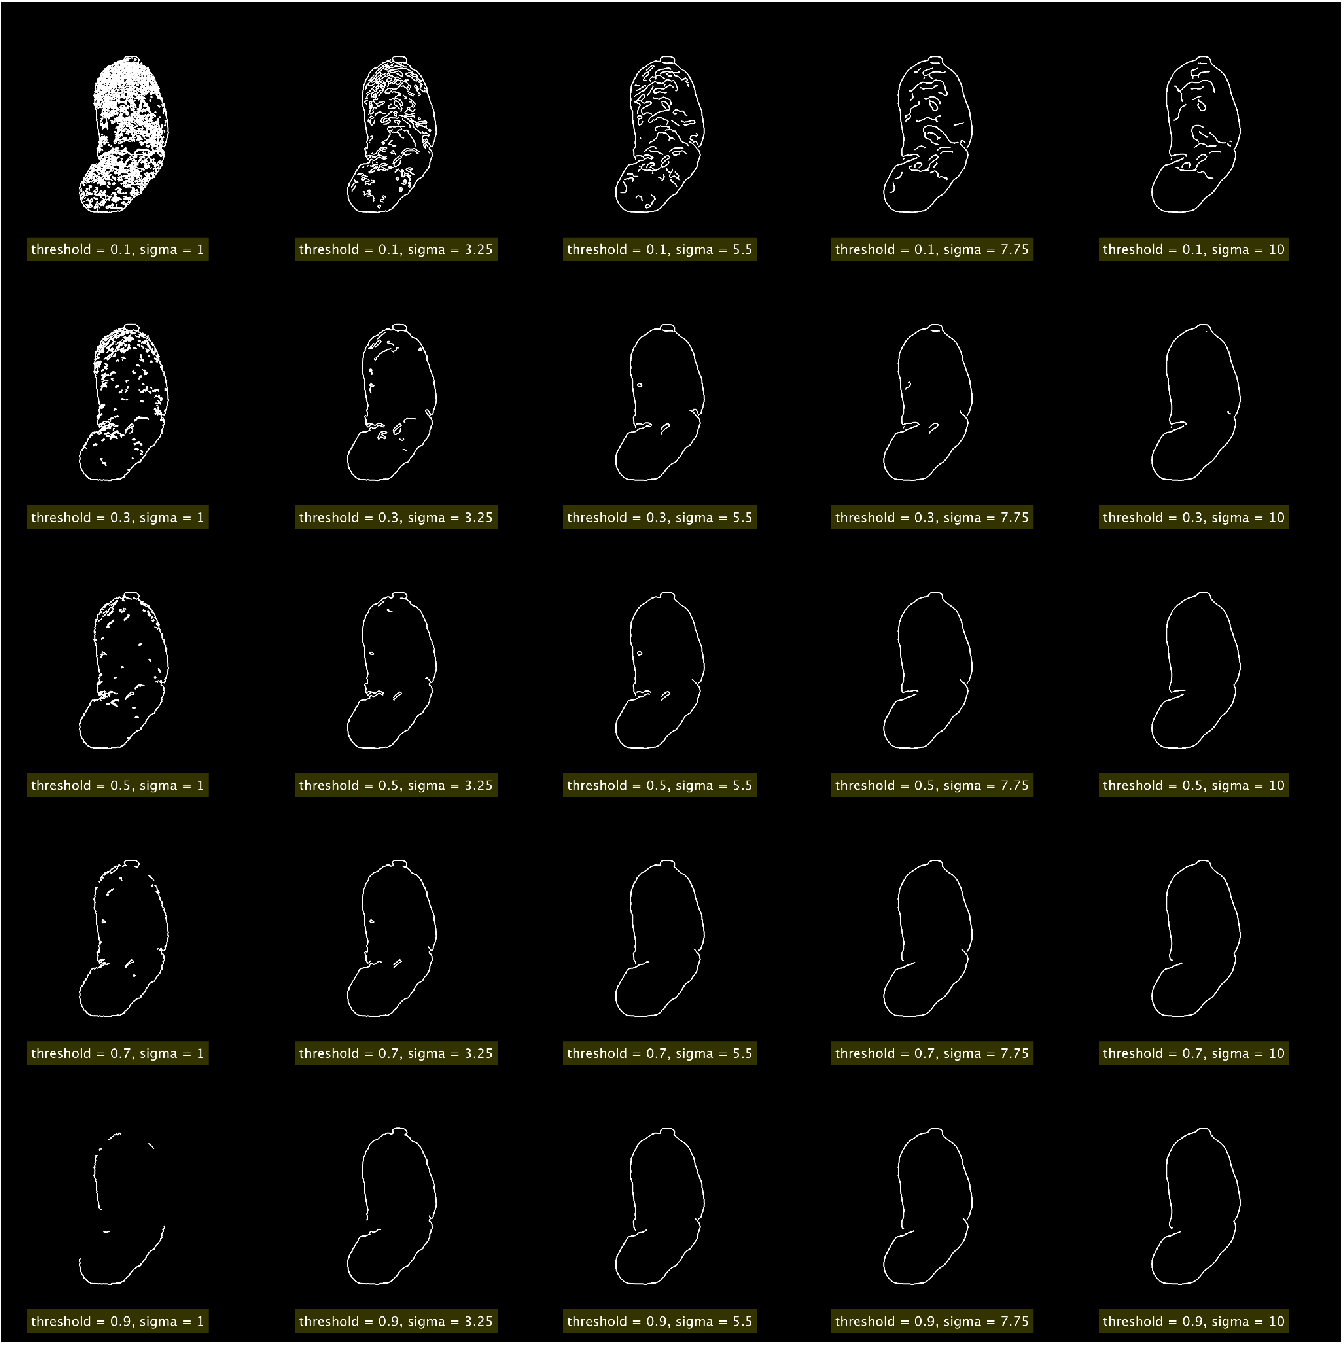
\includegraphics[width = \textwidth]{fig/tiled_canny_test.png}
    \caption{25 Examples of Canny Parameters and Impact on Edge Detection}
    \label{fig:tiled_canny}
\end{figure}
\begin{wrapfigure}[11]{l}{0.4\textwidth}
    \centering
    \captionsetup{justification=centering}
    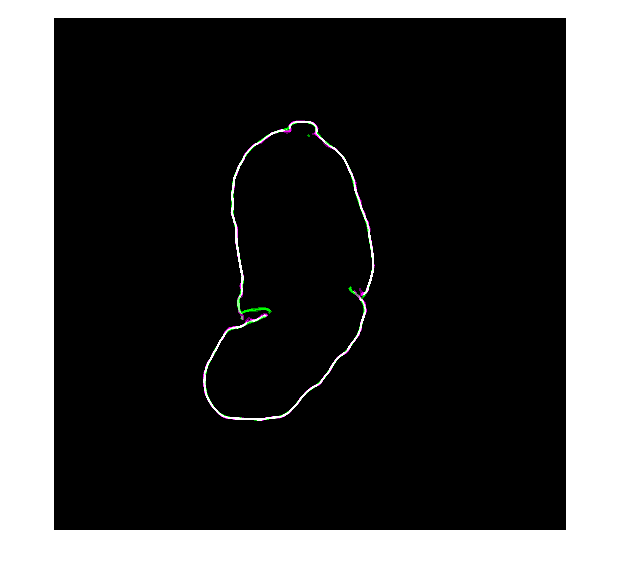
\includegraphics[width = 0.4\textwidth]{fig/overlay_canny_correctparameters.png}
    \caption{Four Edge Results Overlaid in Image Space}
    \label{fig:overlay}
\end{wrapfigure}
In order to capture the edge, the Canny operator was tested for effectiveness over many threshold and standard deviations. Examples of these results are given in Fig. %\ref{fig:tiled_canny}, 
which present the extremes that the function is capable of capturing from the typical asteroid image. The selected values for edge processing were T=0.5 and $\sigma$ = 5. Combined with the previous thresholding steps that output a flat mask, this operator has no issue identifying an appropriate edge for silhouette finding. After the edge is identified, the points are sorted in unit circle order, beginning at the traditional +x axis and moving counter-clockwise in the (u,v) plane. Each image is subsampled to contain an evenly spaced set of points from the full edge result. This is one way in which the data density is reduced for the purpose of faster processing. The original Canny edge output represents each pixel identified as an edge, which can be thousands of data points. 





Taking the four best results from the Canny investigation above, they are overlaid in Fig. %\ref{fig:overlay}, 
to show that differing parameters still provide similar results. The difference between each output is only measured by a few pixels, therefore it can be assumed that the ultimate shape results will not be majorly affected by changing the Canny parameters, as long as the parameters implemented have met the original requirement of identifying only the silhouette and excluding internal features. 

After identifying the silhouette in the image frame and thus in the 3-D camera frame with the addition of the range dimension, the points must be translated into the 3-D body frame which is predefined and known prior to processing. This is an assumption made based on the expected capability to obtain lightcurve information both on the ground and early in the flight plan which will inform about the spin pole and allow for a definition of the body frame to be made. However, for the purposes of this work, the body frame is accessed via SPICE and from scientific convention {Fujiwara2006}{Scheeres2006}.This transformation allows each image to be considered in the body frame against one another, which is what enables the ray trimming process. The points are extended towards and away from the camera direction with the center of the ray corresponding to the originally identified edge point. %include figure of points-> 3d points in body frame -> rays in body frame (use two images for 3d ability)
\subsection{Terminator and Limb Discrimination}
\begin{wrapfigure}[10]{r}{0.4\textwidth}
    \centering
    \captionsetup{justification=centering}
    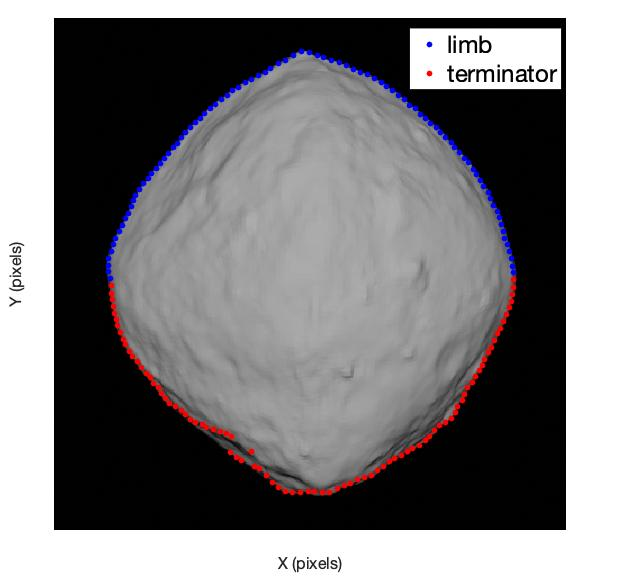
\includegraphics[width = 0.39\textwidth]{fig/limb_term_bennu_correct.jpeg}
    \caption{Limb and Terminator in Bennu Mission Image}
    \label{fig:limbwterm}
\end{wrapfigure}
One major known quantity in any space mission is the direction of the sun vector. This is increasingly important for a small body in which the whole shape can be observed along with the terminator, which is dependent on the relationship between the body, the camera, and the sun positions. In this work, it is assumed that there is perfect knowledge of the sun location and thus the unit vector corresponding to the sun direction in the body and image frames. This state allows for a calculation of the phase angle which becomes crucial when differentiating a limb versus a terminator in an image of a body that is only partially lit. The knowledge of the sun unit vector in the camera frame allows for simple vector products to separate the edge points which are facing the sun and the points which are on the opposing side. %add more description here


\subsection{Ray Generation and Trimming}


The silhouettes have been identified and placed in their assumed positions in the bodycentric frame of the target, and now the next step is to extend these points into rays which will concentrically constrain the surface {Mcmahon2018}. The reason why the rays are necessary is that the points themselves may be misaligned, contain outliers, or possibly not hold enough information to solve for a reasonable resolution of the surface. Extending our points into rays which will be trimmed based on intersections and subsampled allows for more detail without requiring more information. 

%\begin{figure}[h!]
%    \centering
%    \begin{subfigure}[b]{0.32\textwidth}
%        \centering
%        \vcenter{\includegraphics[width = 0.8\textwidth,height = %1.2in]{figures/edge_points_1image.png}}
%        \caption{Original Edge Points in Camera Frame}
%    \end{subfigure}
%    \hfill
%    \begin{subfigure}[b]{0.32\textwidth}
%        \centering
%        \vcenter{\includegraphics[width = \textwidth, height = %1.5in]{figures/one_rays.png}}
%        \caption{Rays: One Image}
%    \end{subfigure}
%    \hfill
%    \begin{subfigure}[b]{0.32\textwidth}
%        \centering
%        \vcenter{\includegraphics[width = \textwidth, height = %1.5in]{figures/two_rays.png}}
%        \caption{Rays: Two Images}
%    \end{subfigure}
%    \caption{Ray Population Process}
%    \label{fig:intensity}
%\end{figure}

The rays are described using a line equation to characterize them in 3D body frame space. The equation of the line segments is as follows for i number of rays $l$ in each view. 
\begin{equation}
    l_i = l_{i,0} + \eta L \hat{r}
\end{equation}


In the above equation, $l_{i,0}$ is the initial point of the ray, $\eta$ is the scale factor from 0 to 1 describing how far along the rays length it's been trimmed (between 0 and 100 percent), L is the length of the pretrimmed ray, and $\hat{r}$ is a generic unit view direction. For this investigation, the original ray length L is set to 2km, centered at the identified edge point and extended towards and away from the camera for limb points, with terminator points at a slight rotation proportional to the phase angle. The $\eta$ factor is calculated after finding all intersections between each limb plane and trimming each ray down to it's likely surface section, and this procedure will be described in later sections.
\begin{wrapfigure}[12]{l}{0.5\textwidth}
    \centering
    \captionsetup{justification=centering}
    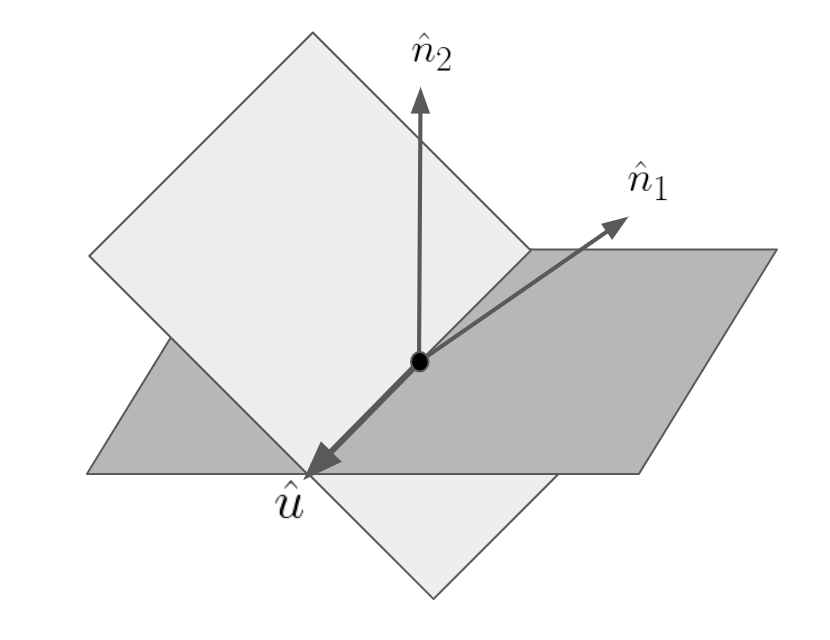
\includegraphics[width = 0.5\textwidth]{fig/planes_intersect.png}
    \caption{Geometry of Two Intersecting Planes}
    \label{fig:two_intersect}
\end{wrapfigure}
\\With a sample of $N_p$ edge points, there can be $N_p$ number of planar quadrilaterals formed by connecting each adjacent edge point as seen in Fig. 
%\ref{fig:twoplanes}
, and calculating its surface normal direction with the following equation:
\begin{equation}
\hat{n}_k = \frac{\hat{r} \times (l_{i+1,0} - l_{i,0})}{|\hat{r} \times (l_{i+1,0} - l_{i,0})|}
\end{equation}



The planar quadrilaterals will be referred to as patches in the following discussion. These patches have an associated normal vector, and two rays which describe the lines in the $\hat{r}$ direction. Processing this information in a batch method, all of the rays are iterated through to find where each plane intersects with another plane from the found silhouettes. The locations of the intersection, along with the percentage along the ray that the location is identified, are saved and then evaluated to find where the rays need to be trimmed away. The line of intersection between two planes in 3D space exists if the cross product of the two normal vectors associated with each plane is nonzero. If $n_1 \times n_2 = 0$, then the two planes in question are parallel and will be ignored. In the implementation presented here, the threshold for a nonzero parallel evaluation is that the magnitude of the cross product of the normal vectors is above $1\times 10^{-10}$. The line of intersection itself also lies along the cross product of the two normal vectors. If an intersection can be found, the $\eta$ value corresponding how much of the line should be kept is saved, and the rest of the line is trimmed and the equation of this specific line is updated to go between $\eta$ length and the other remaining end for the next iteration. Now the direction vector of the intersection line can be founds using the normal vectors of the two planes, as shown in Eq.3. The variable $m$ gives the direction of slope, and a point on the line is found numerically, which corresponds to b, and from there a whole line equation is given in $y = mx + b$ form. 
\begin{equation}
    m = \frac{\hat{n}_1 \times \hat{n}_2}{|\hat{n}_1 \times \hat{n}_2|}
\end{equation}

%now describe the trimming procedure

The results from the line intersection calculations are many line equations describing the unit vector corresponding to the direction of the intersection line, the end points of the original rays, and the points corresponding to the physical end of the intersection line for these finite patches. The next step is to evaluate which parts of the ray must be trimmed away based on the identification of a crossing, and which portions of the ray are kept. 
%above I need to include some math corresponding to the trimming procedure - the trim happens where the normal vectors switch signs along the intersection rays ????
\begin{figure}
    \centering
    \begin{subfigure}[b]{0.49\textwidth}
        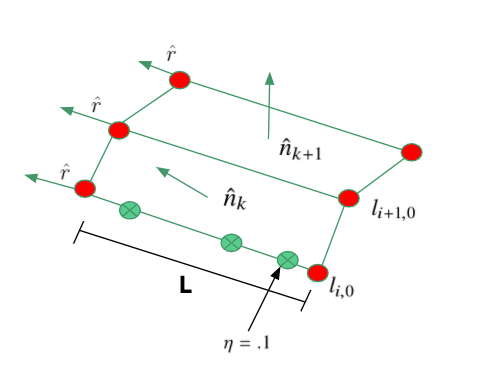
\includegraphics[width = \textwidth]{fig/twoplanes.png}
        \caption{Two adjacent edge planes with sampled points along the line of length L}
    \end{subfigure}
    \hfill
    \begin{subfigure}[b]{0.49\textwidth}
        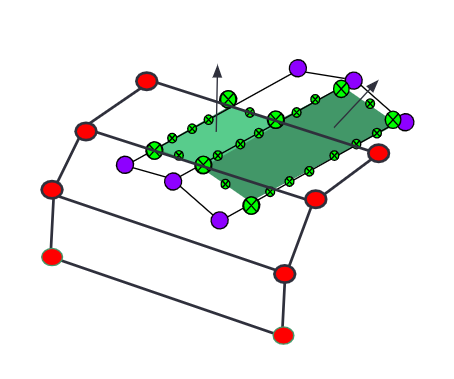
\includegraphics[width = \textwidth]{fig/intersecting_planes.png}
        \caption{Planes and their associated normal vectors: Two observations}
    \end{subfigure}
    \caption{Geometric Depiction of Patch Crossing Calculations}
    \label{fig:twoplanes}
\end{figure}
The algorithm sorts the points along the intersection ray based on the percent along the ray which they fall, and then locates where the calculated projected normal directions switch in sign. This switch is the indicator of an intersection with another limb patch, and therefore serves to show where the ray must be trimmed.
In Fig.%\ref{fig:line_pts}, 
the point identified is $20\%$ along the intersection ray, with a positive normal direction. The point which will delineate the trimmed portion of the ray is at $50\%$ along the original ray, where the surface normal vectors have switched. The derivation of a surface normal direction is crucial for the process of delineating which points intersect on the body and which points intersect off the body and therefore should be discarded. The points that theoretically constrain the surface are what's left after a ray has been processed to find intersections meant to eliminate the points that extend too far. 
\\ As the views are iterated over, the plane intersections are examined and a check is performed to find out if the plane segments are on the inside or outside of the silhouette using the calculation of the surface normal from Eq.3. The segments that are kept are not intersected at all, and therefore must represent our knowledge of where the surface is depending on the resolution of our observation data. As shown in Fig.%\ref{fig:twoplanes},
 one view overlaps with another view and two patches are found. One patch is formed from coplanar limbs and the green points represent the intersections saved. The other patch only intersects the first view on one side, so only one side of the original limb gets trimmed down and resampled. Both of the resulting patches, shown by the green planes, have new normal directions based on the normal directions of the limbs that were intersecting to form them. 
\begin{wrapfigure}[7]{r}{0.5\textwidth}
    \centering
    \vspace{-10pt}
    \captionsetup{justification=centering}
    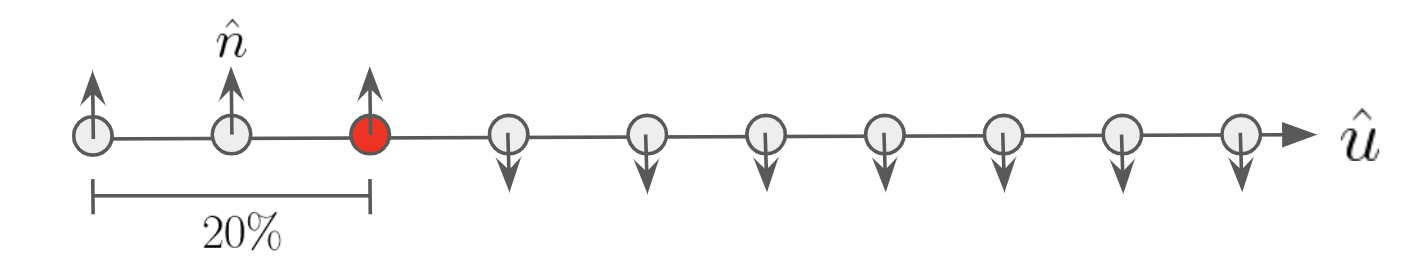
\includegraphics[width = 0.5\textwidth]{fig/line_pts_norms.png}
    \caption{Intersection Ray from Two Patches - Ten Sampled Points and Associated Ray Normals}
    \label{fig:line_pts}
\end{wrapfigure}
\indent After iterating through each view and trimming off the pieces of the rays that become intersected by another silhouette, the algorithm saves the remaining points as a point cloud output result. The segments of the original ray that are kept are the ones that were never intersected. This evaluation is strict and a misidentified edge point could result in the trimming of necessary and correct surface data. This drawback is kept in mind during the tuning procedure of the Canny edge detection function, which is designed to be the least sensitive and therefore refined to only identify true edge points. Depending on the range of the observations about the target body, the surface can be resolved to different magnitudes. It is possible to localize using single-view geometry because of the assumption that range is known. Without this assumption, a multiple-view refinement of location using the coordination of edge points along epipoles within the image frame would be required. This estimation capability can easily be implemented in future iterations of this work in order to reduce assumptions and provide further autonomy to the method. However, in the scope of this work, it is assumed that the attitude and range are known quantities for our spacecraft. If a full equatorial survey is able to be conducted, the resulting model will have more data and thus can be further refined by our method compared to a survey with less frequent observations taken. In the test cases presented in this paper, simulated data was used to represent an optimal scenario of observational ability. Using Blender {blender}, the case of a $0^\circ$ phase angle could be simulated for maximum limb brightness and the elimination of a terminator. Data sets were collected for both Itokawa and Bennu, to examine the individual challenges of mapping an irregular shaped body versus a symmetric body. 

\subsection{Outlier Rejection Scheme}
Once the limb rays have been iterated on and their final intersections have been trimmed down, the remaining points and their associated surface normal directions are saved as 3D data suitable to represent a point cloud. In order to reconstruct a surface from the points, we first have to sample down the number of resultant points in order to eliminate outliers from a coarse trimming bias and promote a smoothing of the final surface {Pomerleau2013}. We also implement a function to filter out noisy particles {Rusu2008}. This function keeps any points that have 10 neighboring points within 1 standard deviation of the mean distance between all points in the point cloud.

\subsection{Surface Reconstruction with Ball-pivoting}

Solving for the final surface involves implementing a method that calculates triangular facets and their associated normal unit direction. The method implemented in our work is a ball-pivoting approach that results in a completely closed manifold. The ball-pivoting method forms a closed shape from a point cloud using a ball with a pre-specified radius $\rho$. A triangular face is formed if the ball, initialized at a random point, contains no more than three points {Bernardini1999}. This ball moves along the edges of the triangles solved until it has reached every point available. From there, Delaunay triangulation is applied to find the optimal vertices for each facet and connect the shape as it would fit over a closed volume, as one would expect for a small body {DiAngelo2011}. These methods for reconstruction were chosen because of their geometric simplicity and their restriction to form a closed surface which is a requirement for any small body target. As shown in Fig.\ref{fig:twosurfaces}, we capture some of the finer details of the shapes despite the lower resolution of the limb-based method. 
\begin{figure*}[ht!]
    \centering
    \begin{subfigure}[t]{0.5\textwidth}
        \centering
        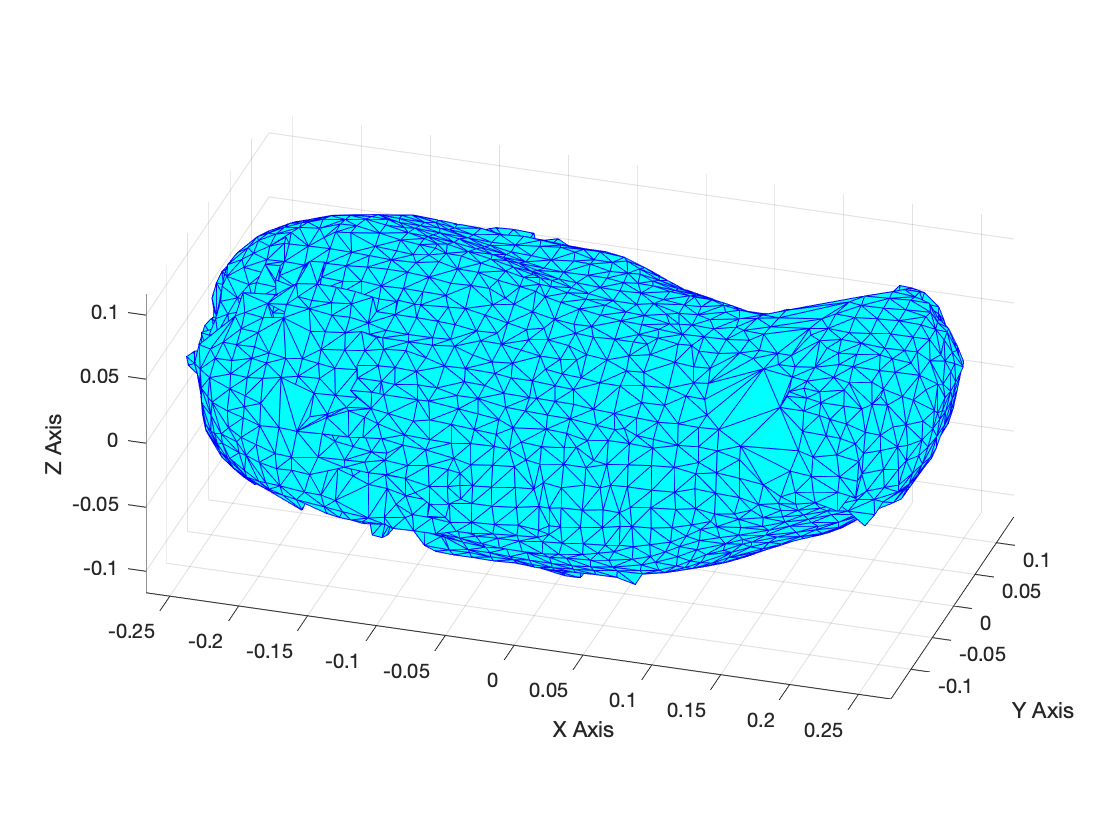
\includegraphics[width = 1\textwidth]{fig/itokawa_recon.png}
        \caption{Itokawa Surface Result}
    \end{subfigure}%
    ~ 
    \begin{subfigure}[t]{0.5\textwidth}
        \centering
        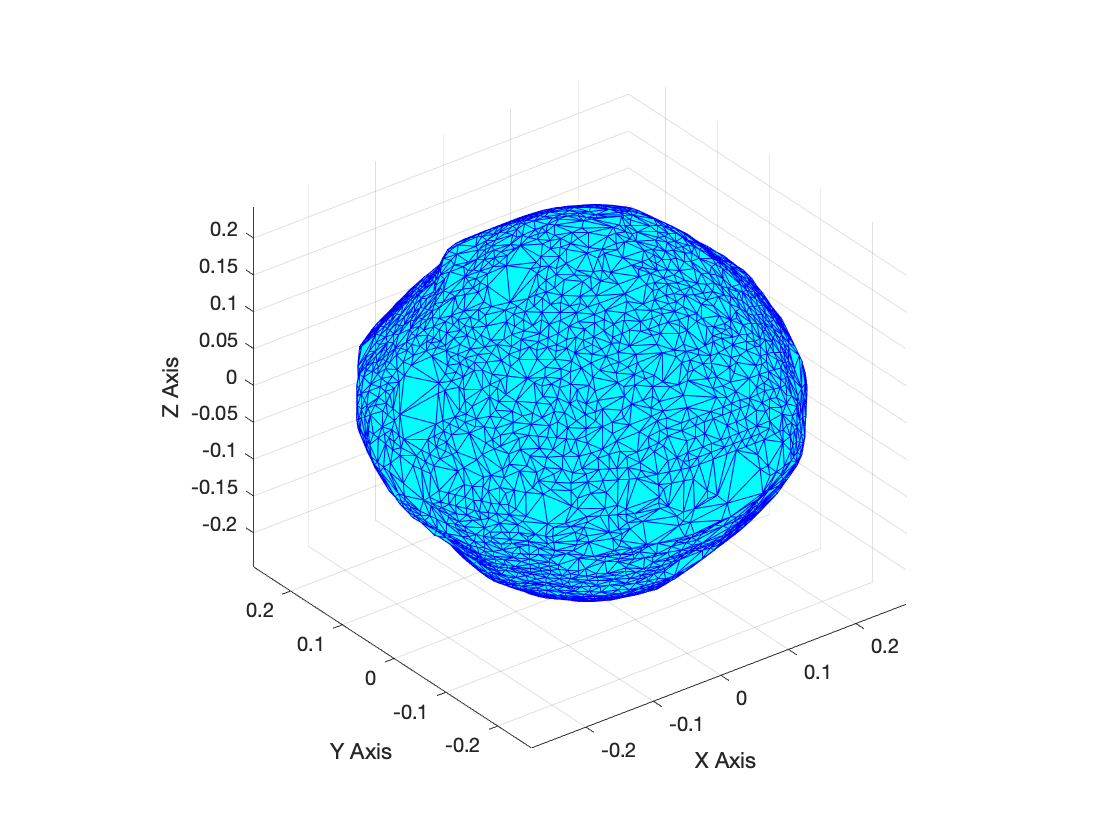
\includegraphics[width = 1\textwidth]{fig/bennu_recon.png}
        \caption{Bennu Surface Result}
    \end{subfigure}
    \caption{Ball-Pivoting Surface Reconstruction Results of Itokawa and Bennu Point Clouds}
    \label{fig:twosurfaces}
\end{figure*}
\section{Shape Results}
\subsection{Simulated Data}
Using 21 simulated images of Itokawa and 11 images of Bennu, spaced $33^{\circ}$ apart along both the equator and prime meridian of the bodies, generated in Blender{blender}, we were able to resolve the following point clouds and the resultant closed mesh. We also report the shape model's relative error compared to a high-resolution models of Itokawa and Bennu made using SPC {Gaskell2006} from the Hayabusa and OSIRIS-REx missions, respectively. This error is calculated using a per vertex geometric distance between the measured mesh (built using iterative limb-trimming) and the reference mesh, or the detailed, high-resolution Gaskell models. We find that both models are extremely close to the truth, with error on the order of meters. Compared to more-precise methods that fit landmark data to maplets, our method gives similar results. The point-cloud post-processing steps are able to reduce the artifacts leftover from limb-trimming, typically observed as lines across the final surface. However, we would like to reduce the dependence on post-processing in future works for the sake of retaining information about smaller features that our current algorithm was not refined enough to pick up, such as large boulders on Bennu.
\begin{figure*}[ht!]
    \centering
    \begin{subfigure}[t]{0.4\textwidth}
        \centering
        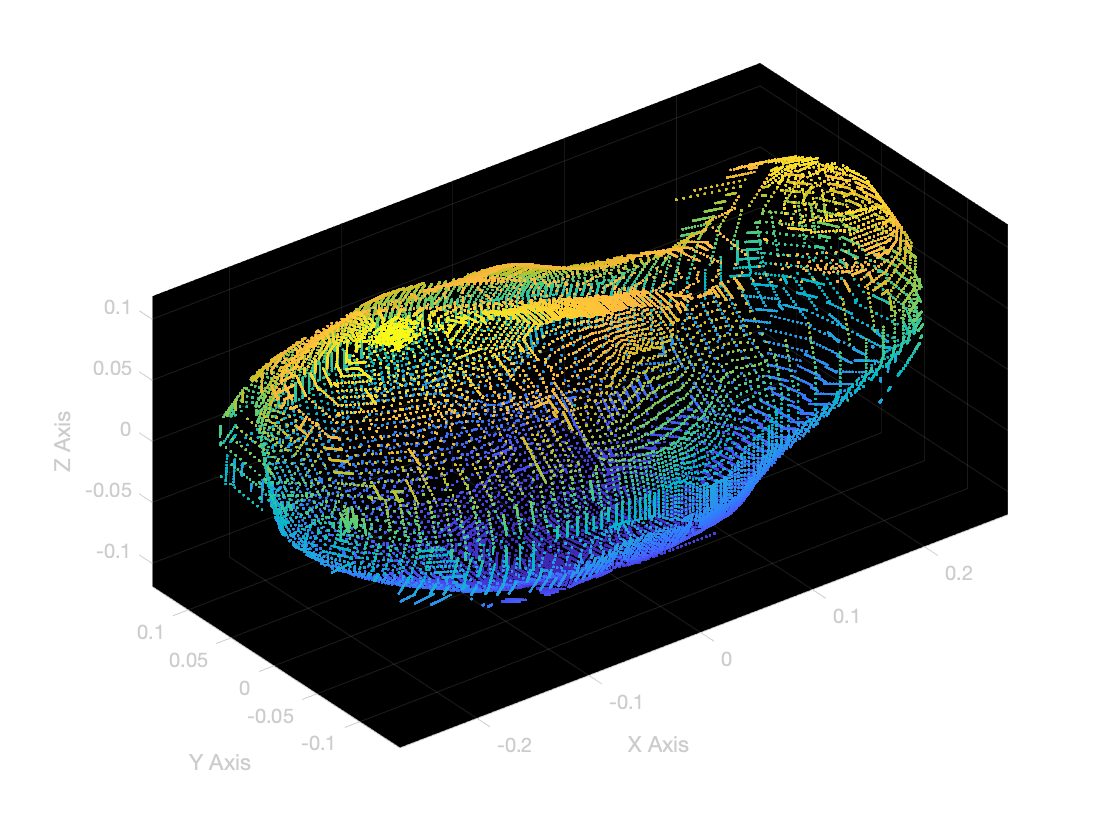
\includegraphics[width = \textwidth]{fig/dense_itokawa.png}
        \caption{Original Point Cloud}
    \end{subfigure}%
    \begin{subfigure}[t]{0.4\textwidth}
        \centering
        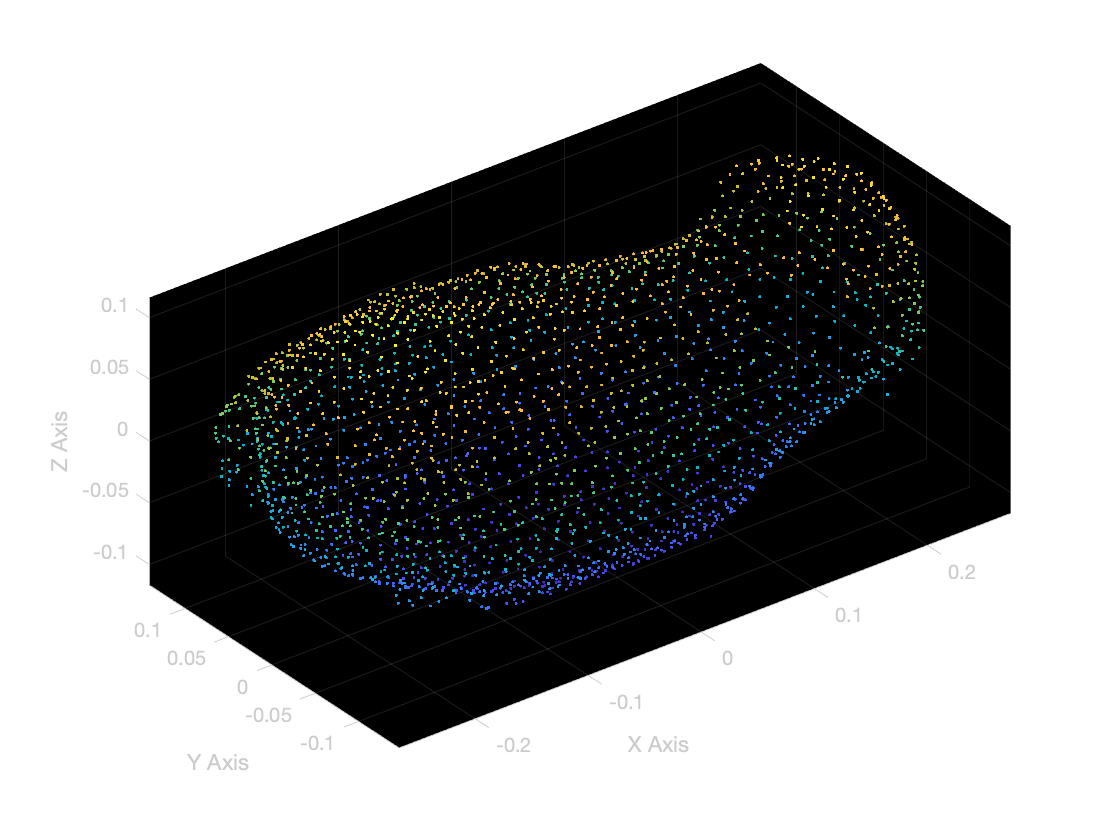
\includegraphics[width = \textwidth]{fig/sparse_itokawa.png}
        \caption{Sub-sampled and Noise Reduced Point Cloud}
    \end{subfigure}
    \caption{Pre- and Post-Processed Point Cloud of Itokawa Limb-Trimmed Shape}
\end{figure*}

The reconstruction of Itokawa based on 21 simulated images is shown in Fig.\ref{fig:itokawa_error}. The resultant shape is overall smooth along the surface, the concavities in the structure have been captured well based on the data survey, and the error in the shape when compared to a high-resolution model is between -22 and 33 meters, with an average surface error of -3 meters. The longest dimension of Itokawa is approximately 535 meters, which means that the body could be mismodeled up to 6 percent. The map shows that areas around the intersection with the x-axis present the most negative surface errors. This is believed to be caused by an assumption made about the rays extending from the camera frame to the edge of the body. The calculations described in previous sections assume that $\hat{u}$ are straight, parallel when traced from the body to the camera. However, the images were captured at a relatively close distance where this assumption cannot hold without repercussions in the final shape. A better modeling technique would be to consider the line-of-sight vector from the center of the camera frame to the edge of the body, which extends as a cone shape. 


\begin{figure}[h!]
    \centering
    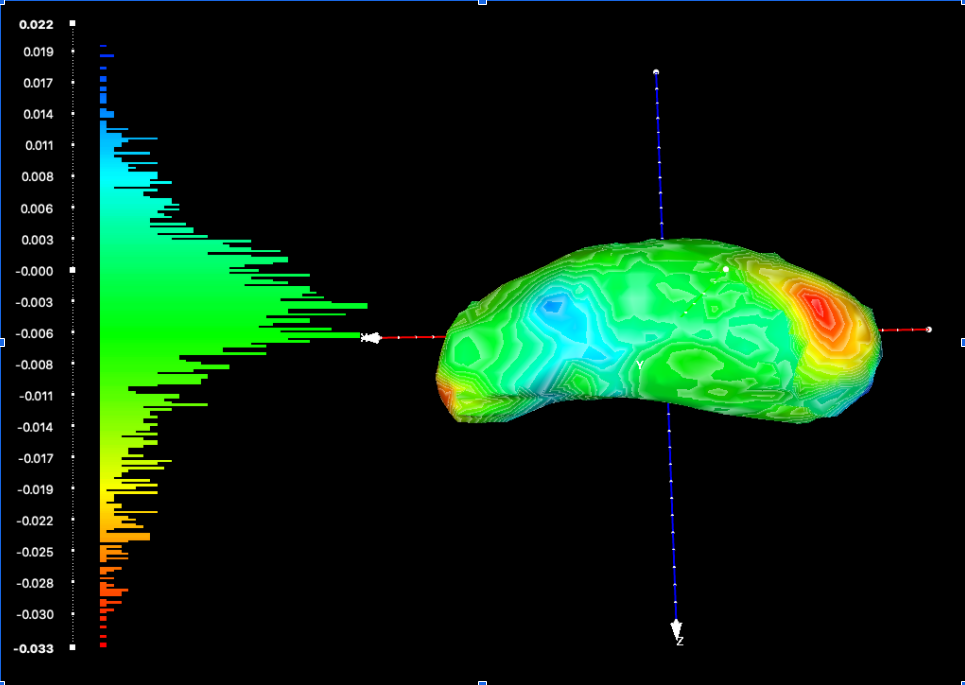
\includegraphics[width = 0.7\textwidth]{fig/itokawa_sim.png}
    \caption{Limb-based Itokawa shape compared to SPC, with surface error in units of kilometers}
    \label{fig:itokawa_error}
\end{figure}


\begin{figure*}[h!]
    \centering
    \begin{subfigure}[t]{0.5\textwidth}
        \centering
        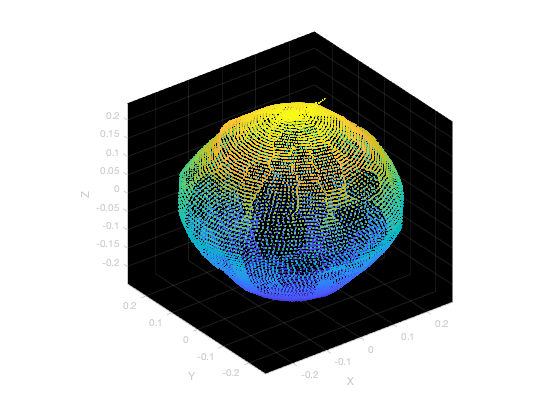
\includegraphics[width = \textwidth]{fig/dense_bennu.png}
        \caption{Original Point Cloud}
    \end{subfigure}%
    \begin{subfigure}[t]{0.5\textwidth}
        \centering
        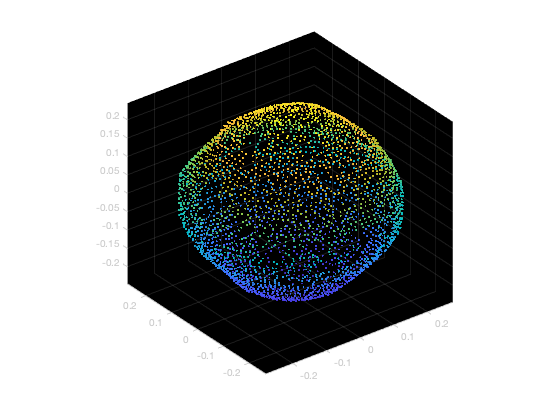
\includegraphics[width = \textwidth]{fig/sparse_bennu.png}
        \caption{Subsampled and Noise Reduced Point Cloud}
    \end{subfigure}
    \caption{Pre- and Post-Processed Point Cloud of Bennu Limb-Trimmed Shape}
\end{figure*} 

The model shown here, developed using 11 images of Bennu along it's equator, is also a comparable shape result when measured against high-resolution models such as the 75cm surface model developed using observations made by OSIRIS-REx. The error found using the per-vertex geometric measuring approach is between -2.1 and 2.0 meters, with an average error of 0.5 centimeters. With the largest dimension of Bennu measuring at 565 meters, this represents a maximum mismodeling of 0.4 percent. This model has no predictable areas of under or over-estimation. The resulting shape is smooth, captures the size and general shape of the body, and could easily be used in any proximity navigation solutions. Using data from a relatively close range, we expected the same perspective errors as were found in the Itokawa model, however, the simple convex shape of Bennu was easily and accurately mapped using it's silhouette.  


\begin{figure}[h!]
    \centering
    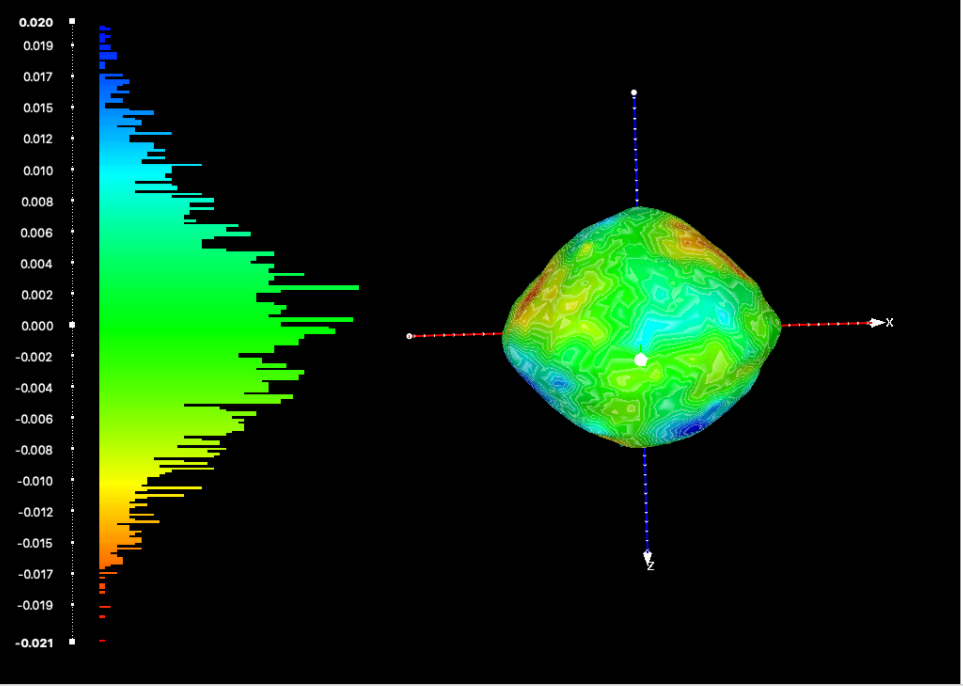
\includegraphics[width=0.75\textwidth]{fig/bennu_sim.png}
    \caption{Limb-based Bennu shape compared to SPC, with surface error in units of kilometers}
    \label{fig:bennu_error}
\end{figure}


\subsection{Shape Modeling from Mission Data}
The last limb-trimmed shape model presented is developed using real mission images taken during the approach phase of the OSIRIS-REx mission by the PolyCam instrument. The major factor differentiating the previous simulated data models from the following model is the appropriateness of the zero degree phase angle assumption. For these reconstructions, we found views that had a low phase angle and therefore could easily ignore the terminator when searching for edge contours in the images without propagating large error in the model. It is to be expected that ignoring the phase angle between the sun and the body will always cause an under-determination of the shape by assigning the terminator as sunlit limb points. This drives forward future work in delineating terminator and limb from varying phase angles, however, the model presented here works under the assumption that the body is always lit from behind the direction of the camera. 

Implementing the same procedures as shown in previous sections, we were able to process 70 images of the asteroid Bennu using Canny edge detection for the silhouette identification and limb-trimming for shape resolution in order to build a surface model from these initial silhouette points. The results show that the model is biased towards underestimating the size of the surface, with the error spanning from -55 to 7 meters, and a mean error of -7 meters. As predicted, the phase angle assumption caused terminator points to be associated with the edge, therefore reducing the size estimate of the body as a whole based on the trimming scheme. However, the shape is reasonably captured based on the dimensions of Bennu and could be used for initial navigation when better data is not yet available.  

\begin{figure}[H]
    \centering
    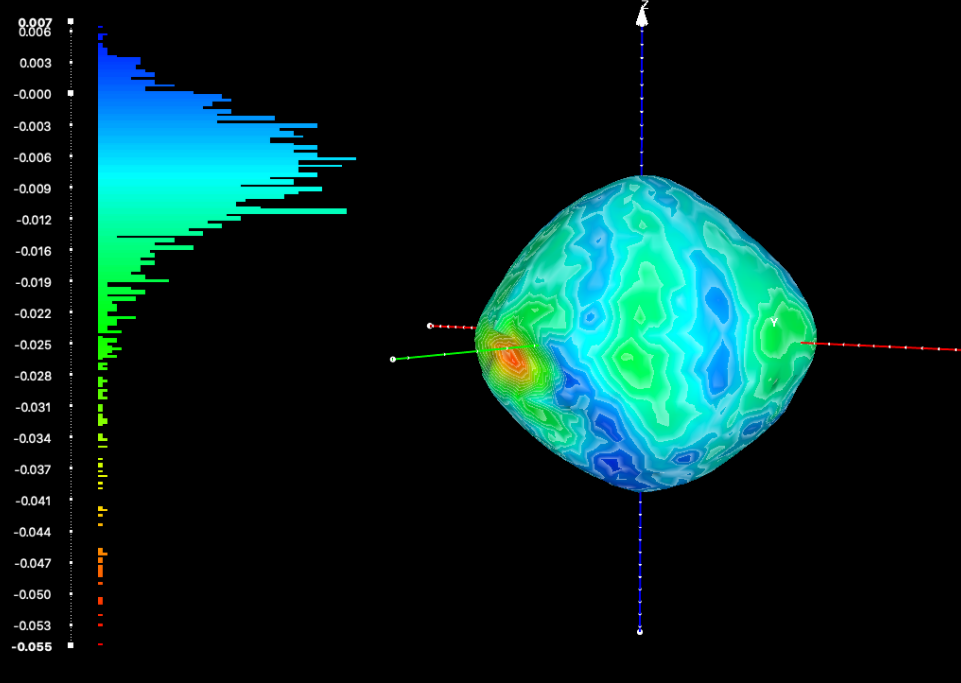
\includegraphics[width = 0.8\textwidth]{fig/bennu_real.png}
    \caption{Bennu Shape Model from Real Images, compared to SPC, surface error in kilometers}
    \label{fig:bennu_real}
\end{figure}


\section{Matching Localization with Normalized Cross-Correlation}
\subsection{Methods}

The step of localization is important for any autonomous system to be able to navigate with the onboard generated map without human interference. Keeping a record of images with known locations about the body is one way to inform your future observations of their current orientation and range. We show a simplistic localization method based on finding correlations between test images and a library of images which were collected to build the initial model. With the asteroid Itokawa as our model, we use the Hayabusa mission image set from Oct. 1st, 2005 as the test images. The goal was to provide a test image with an associated latitude and longitude, and find the highest correlation score between this test image and the set of library images previously saved. Ideally, the highest correlation score would correspond to the same latitude and longitude between the test and library image. The process of correlation followed a simple iteration scheme where each test image was measured for a correlation score between each library image. We used a set of 36 library images of Itokawa generated in Blender with varying longitudes, spanning every 10 degrees. This library was acceptable for the images taken on approach, seeing as both the test images and the library set only greatly varied in the longitude orientation due to the spacecraft approaching the target body at an angle perpendicular to the spin axis on the day that the data was taken. 

The correlation score is an important quantitative measure of similarity between images. This value, r,  was measured between two binary images, and falls between 0 and 1, with 0 meaning no correlation between the images, and 1 meaning that the images have exactly the same pixel values for each location. The score used in this study was calculated as follows:
\begin{equation}
    r = \frac{\sum\limits_m \sum\limits_n (A_{mn} - \Bar{A})(B_{mn} - \Bar{B})}{\sqrt{\big ( \sum\limits_m \sum\limits_n (A_{mn} - \Bar{A})^2 \big ) \big( \sum\limits_m \sum\limits_n (B_{mn}-\bar{B})^2 \big)}}
\end{equation}
In the correlation coefficient equation, m and n refer to the u and v axes of the images in question, A corresponds to the test image, B corresponds to the reference image, while $\bar{A}$ and $\bar{B}$ refer to the two-dimensional mean of the pixel intensities in image A and B, respectively. The images in both the test set and the library were all 1024x1024 pixels. No stars were obvious in any of the test images, however, the test image corresponding to $89^{\circ}$ was found to be flat.

\subsection{Results}
Correlating two images based on pixel values has proven to have some promise, however, our approach did not successfully match test images to the correct corresponding library image. The test case based on the asteroid Itokawa has shown that the body exhibits symmetries along certain axes that make it difficult for this correlation method to match the correct longitudes. We have learned that high correlation scores are possible between images that are meant to be matched, which shows that the 2-D correlation coefficient can see some similarities between images taken at the same longitudes. If this method were to be applied for localization procedures, it would need more rigorous matching capabilities. Shown in Fig.\ref{fig:expected}, the two images presented are both focused on the same latitude and longitude, both $0^{\circ}$. The corresponding correlation coefficient is above 0.9, which means these images are a strong match to each other. However, the iteration scheme found another image in our library with a higher matching score and associated our test image with the incorrect image shown in Fig.\ref{fig:highest}. 

\begin{figure}[H]
\centering
    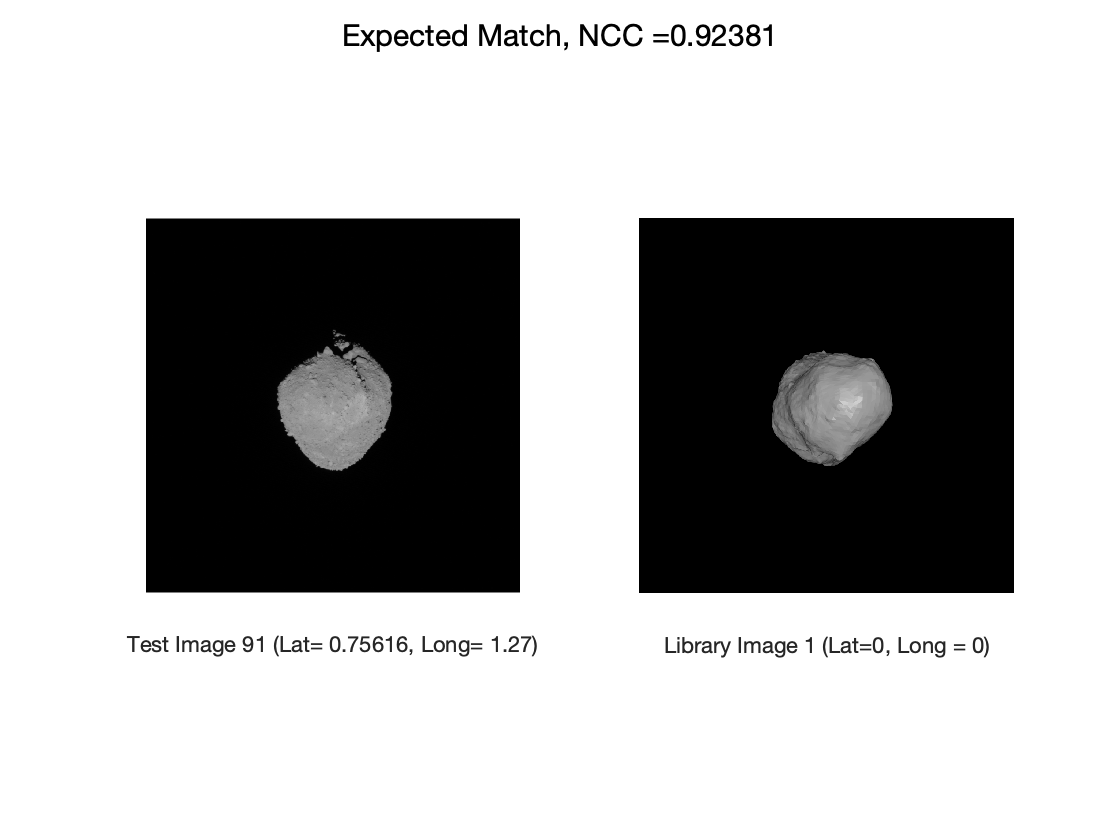
\includegraphics[height=0.43\textheight]{fig/expected_match.png}
    \caption{Test image and Library Image, Expected Match Pair}
    \label{fig:expected}
\end{figure}
\begin{figure}[h!]
    \centering
    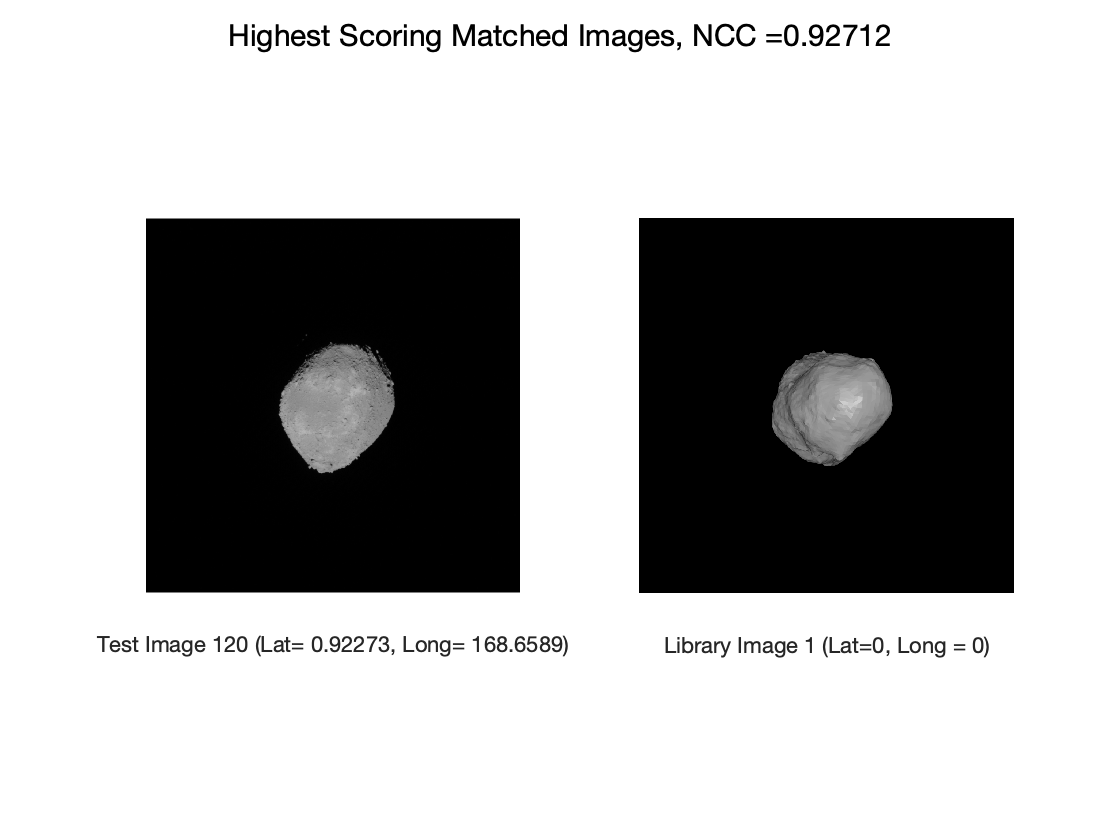
\includegraphics[height=0.43\textheight]{fig/highest_score.png}
    \caption{Test Image and Library image, Actual Match Pair}
    \label{fig:highest}
\end{figure}

We can see from these comparisons that the algorithm failed to account for rotations in the body orientation. The expected match and the actual match have correlation scores within 0.005 of each other, showing that the algorithm can still correlate similarities well. However, this cannot be claimed as a success for navigation purposes seeing that the error in the matched longitude is $168.66^{\circ}$. Further analysis shows that for all of the images in the library, the score of the correlation between the library image and a test image follows a symmetric pattern, shown in Fig.\ref{fig:heatmap}. If this method of localization was successful and we could match test images to their correct library equivalent, we would see the highest correlation scores following a $y=x$ trend across the score map. The observations made instead show that the highest correlation scores follow the symmetry of the body, and the most likely match in the images are when the asteroid is being viewed from the $0^{\circ}$ and $180^{\circ}$ orientations. This data could be improved with further centering of test images during pre-processing, testing flipped orientations of the library images, or possibly examining the silhouette only for localization. Another avenue of testing could be for lighting-condition invariance, where many phase angles are tested and machine learning is applied to match features despite different sun angles \citep{Manni2020}. 

\begin{figure}[H]
    \centering
    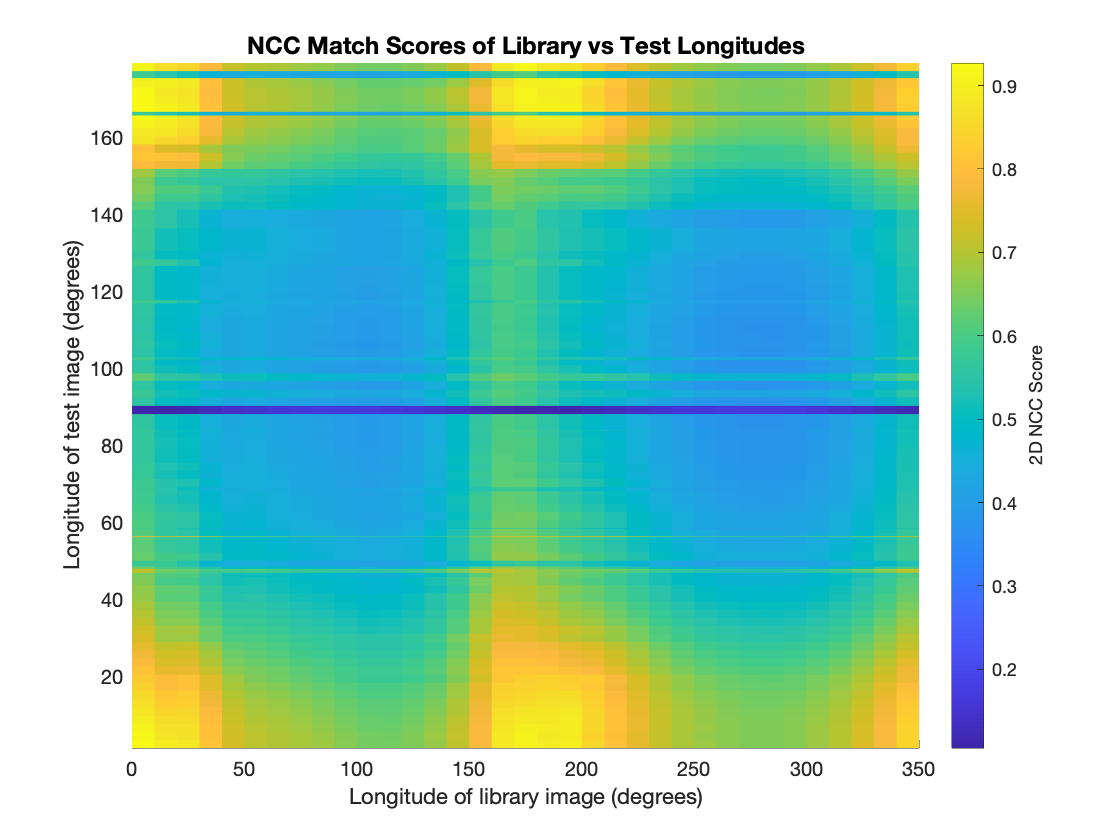
\includegraphics[width= 1.1\textwidth]{fig/all_scores.png}
    \caption{2D Correlation scores between all library images and all test images, based on longitude}
    \label{fig:heatmap}
\end{figure}

\section{Analysis}
\subsection{Error Evaluation}
The models generated with the limb-trimming method have been compared to mission-derived truth models of the same bodies. The 101955 Bennu shape model used for comparison is sourced from data during the approach phase of the OSIRIS-REx mission, and was made available publicly in November 2018{}. This model has a resolution of 6m over the surface. The 25143 Itokawa shape model used for comparison is the Gaskell shape model produced with Hayabusa with a resolution of 49,152 facets \citep{Gaskell2004}. A surface comparison between two shape models is performed using a Distance from Reference Mesh function, which calculates the closest distance from the reference mesh, or truth model, to the measured mesh, which is the model produced via limb trimming. The distance is left signed to appropriately characterize under- or over-estimated volumes. 


% \begin{table*}[h!]
% \centering
%      \begin{tabular}{|c||c|c|c|c||c|c|}
%      \hline
%      \multicolumn{1}{|c||}{}&
%      \multicolumn{4}{c||}{Point Cloud Dimensions}&
%      \multicolumn{2}{c|}{Surface Reconstruction}\\
%      \hline
%            \textbf{Test Case}& \textbf{$\#$ of Points} & \textbf{x (m)} & \textbf{y (m)} & \textbf{z (m)} & \textbf{Mean Error (m)} & \textbf{RMS (m)} \\
%           \hline
          
%           Bennu Truth Model{Barnouin2019} & 25350 & 563.3& 541.4& 495.5 & N/A  & N/A\\
%           \hline
          
%           \hline
          
%           Itokawa Truth Model%{gaskell_ito} & 24578 & 560.5& 305.3& 243.5 & N/A  & N/A\\
%           \hline
%      \end{tabular}
%      \caption{Comparison of Shape from Silhouette Model Results to Truth Models}
% \end{table*}
\subsection{Boulder Resolution}
With the error ranges seen here, we can expect to model boulders to at least 33 meter accuracy as the worst resolution bounds. Areas with higher accuracy modeling on these shapes can resolve boulders down to 2 meters in diameter. As we have shown in YORP modeling, highly effective radiating boulders (with flat faces) need to be at least 1 meter in diameter to contribute significantly to the global YORP torque. With more realistic shapes such as rounded wedges, this can increase to the tens of meters range.
One major takeaway from previous chapters is that for bodies of the rough diameter of Bennu and Itokawa, the boulders that matter for modeling YORP are 1m in diameter and above, with more emphasis placed on large boulders up to the maximum size of 55m in diameter. In this modeling procedure, we can expect to capture the absolute largest boulder on the surface (in the tens of meters range) which will give a small glimpse as to the boulder-induced YORP torque that could be measured by surface modeling. Higher fidelity surface modeling is the driver of better YORP torque models. As we've examined the boundaries of significance, we show that a well-made shape model is necessary for calculating the accurate YORP torques.

We conclude that we are capable of building a shape model for an irregular as well as a convex body given low phase angle imagery. This shape model was comparable in size and shape to the target body and with improvements, could serve as a reliable data product for navigation in a scenario without reliable surface feature identification methods. This work also tests a preliminary, matching-focused localization method that we would like to integrate into a full navigation scheme with further testing. It has been shown that limbs can serve as reference data for a spacecraft navigating about a body, but that irregularities in the shape can cause major error between the predicted limb locations and the observed limb locations \citep{Liounis}. We would also like to challenge many of our assumptions, such as the low phase angle on approach, perfect knowledge of range and attitude, as well as our fine tuning of the Canny edge detection thresholds. We hope to find ways to iteratively update our model, ingesting new observations after the surface has been constructed, and allowing a transition between low and high resolution mapping methods as a spacecraft finds that better data is available.


